\documentclass{article}
\usepackage[utf8]{inputenc}
\usepackage{graphicx}
\begin{document}
\section{Data Description}
We are working with the Taxi Dataset from before. A Proposition from my last investigation involved dropping all erroneous rows before feature generation began. At this point we have 4566 rows. There are only two erroneous rows still in the dataset which have now been removed so we have 4564 rows. We also drop the missing values leaving 4433 rows.


Next we should drop columns that are irrelevant to clustering. These include:
\begin{enumerate}
\item X
\item X.1
\item error\_count
\item outlier\_count
\item missing\_values\_count
\item not\_store\_and\_fwd
\end{enumerate}

\section{Data cleaning}
to prepare for PCA we need to make sure that data is comparable, some features will not be able to be normalized.
\subsection{Lpep Times}
We should convert this to Unix time, as our algorithm may not be able to correctly interpret this date-time format.
\subsection{One Hot encoding}
For PCA to work well we should one hot encode any remaining text fields. The fields:
\begin{enumerate}
\item VendorID
\item RateCodeID
\item Payment\_type
\item Trip\_type
\end{enumerate}

\section{Feature Generation}
Next we need to generate a handful of features.
\subsection{Actual Velocity}
A very simple value for velocity can be calculated from the distance divided by the journey time in seconds.

\subsection{Price from distance only}
a factor of price without things like added tax and etc, the price only generated from distance. This can be calculated from Total\_amount. As I investigated this i found that Fare\_amount already represents this variable.

\subsection{Normalization}
It is good practice to normalize numerical data where possible before starting PCA so that components are only weighted by value and variance and not size. We need to normalize the following:
\begin{enumerate}
\item Pickup\_longitude
\item Pickup\_latitude
\item Dropoff\_longitude
\item Dropoff\_latitude
\item Passenger\_count
\item Trip\_distance
\item Fare\_amount
\item Tip\_amount
\item Tolls\_amount
\item Total\_amount
\item pickup\_unix
\item dropoff\_unix
\item trip\_time\_seconds
\item velocity
\end{enumerate}
The following were not not normalized:
\begin{enumerate}
\item Pickup\_longitude
\item Pickup\_latitude
\item Dropoff\_longitude
\item Dropoff\_latitude
\item Trip\_distance
\item velocity
\end{enumerate}

\section{PCA Analysis}
\subsection{Eigenvalues and dominant axes}
At this point we have a total of 27 variable.

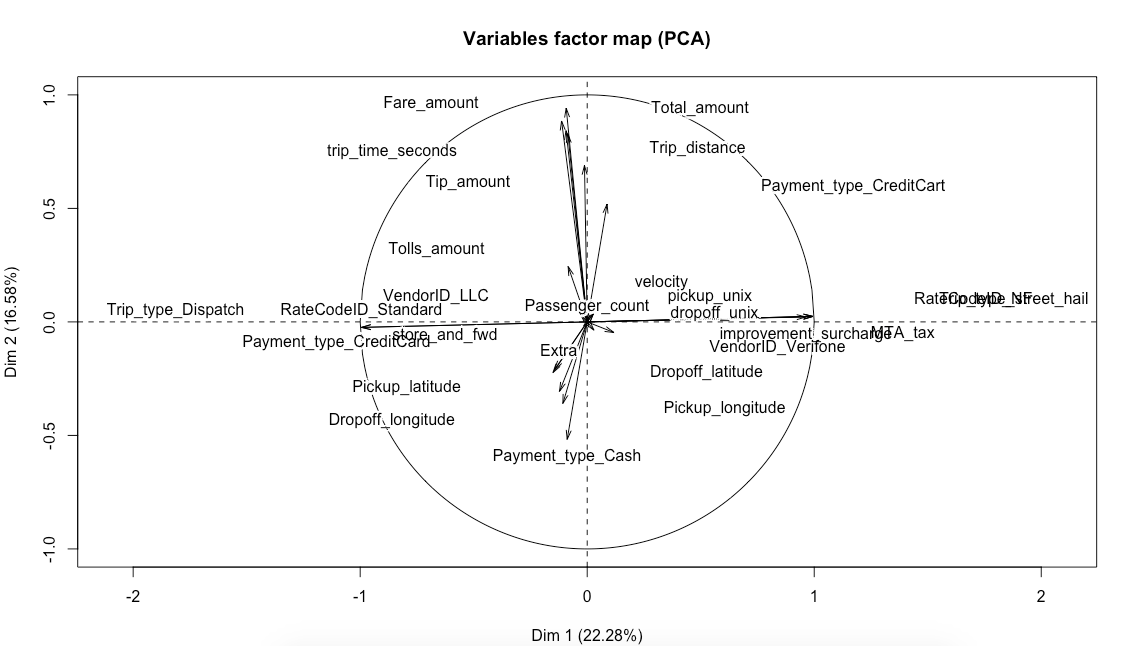
\includegraphics[width=\textwidth]{PCA.png}
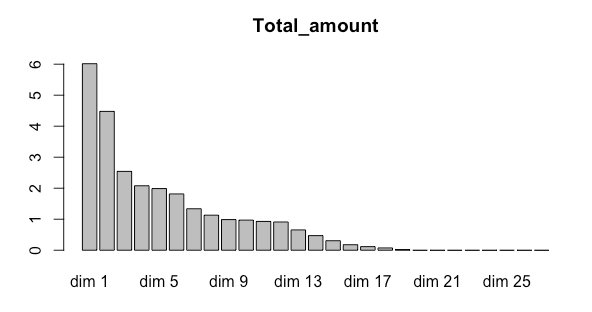
\includegraphics[width=\textwidth]{part1barplot.png}

\label{my-label}
\begin{tabular}{llll}
test & eigenvalue & percentage of variance & cumulative percentage of variance \\
comp 1 & 6.015 & 22.278 & 22.278 \\
comp 2 & 4.478 & 16.585 & 38.862 \\
comp 3 & 2.543 &  9.419 & 48.281 \\
comp 4 & 2.079 &  7.699 & 55.979 \\
comp 5 & 1.987 &  7.361 & 63.340 \\
comp 6 & 1.816 &  6.725 & 70.065 \\
comp 7 & 1.337 &  4.952 & 75.017 \\
comp 8 & 1.131 &  4.189 & 79.206 \\
comp 9 & 0.988 &  3.658 & 82.863 \\
comp 10 & 0.972 &  3.599 & 86.462 \\
comp 11 & 0.929 &  3.441 & 89.904 \\
comp 12 & 0.911 &  3.374 & 93.278 \\
comp 13 & 0.655 &  2.425 & 95.703 \\
comp 14 & 0.470 &  1.742 & 97.445 \\
comp 15 & 0.306 &  1.132 & 98.577 \\
comp 16 & 0.177 &  0.655 & 99.232 \\
comp 17 & 0.115 &  0.425 & 99.657 \\
comp 18 & 0.074 &  0.273 & 99.930 \\
comp 19 & 0.019 &  0.070 & 100.000 \\
comp 20 & 0.000 &  0.000 & 100.000 \\
comp 21 & 0.000 &  0.000 & 100.000 \\
comp 22 & 0.000 &  0.000 & 100.000 \\
comp 23 & 0.000 &  0.000 & 100.000 \\
comp 24 & 0.000 &  0.000 & 100.000 \\
comp 25 & 0.000 &  0.000 & 100.000 \\
comp 26 & 0.000 &  0.000 & 100.000 \\
comp 27 & 0.000 &  0.000 & 100.000
\end{tabular}

\section{Variables point of view}
PCA has reduced our dataset down to 3 dimensions. The below tables describe the strength of these values in each dimension.

\subsection{dimension descriptions Dim 1}
\label{my-label}
\begin{tabular}{lll}
& correlation   &   p.value \\
Trip\_type\_street\_hail   &  0.99386177 &  0.000000e+00 \\
RateCodeID\_NF           &  0.99386177 &  0.000000e+00 \\
MTA\_tax                 &  0.99386177 &  0.000000e+00 \\
improvement\_surcharge   &  0.96381202 &  0.000000e+00 \\
Extra                   &  0.11819145 & 2.909115e-15 \\
Payment\_type\_CreditCart &  0.08758005 & 5.197305e-09 \\
VendorID\_Verifone       &  0.02957182 & 4.897721e-02 \\
VendorID\_LLC            & -0.02957182 & 4.897721e-02 \\
Tolls\_amount            & -0.08399587 & 2.133242e-08 \\
trip\_time\_seconds       & -0.08553300 & 1.172330e-08 \\
Payment\_type\_Cash       & -0.08830664 & 3.876594e-09 \\
Total\_amount            & -0.09260283 & 6.528726e-10 \\
Trip\_distance           & -0.09336012 & 4.729037e-10 \\
Dropoff\_longitude       & -0.10726733 & 8.032696e-13 \\
Fare\_amount             & -0.11297777 & 4.551051e-14 \\
Pickup\_longitude        & -0.12201843 & 3.571623e-16 \\
Pickup\_latitude         & -0.14405064 & 5.492807e-22 \\
Dropoff\_latitude        & -0.15081861 & 5.719633e-24 \\
Trip\_type\_Dispatch      & -0.99386177&  0.000000e+00 \\
RateCodeID\_Standard     & -0.99386177&  0.000000e+00
\end{tabular}

\subsection{dimension descriptions Dim 2}
\label{my-label}
\begin{tabular}{lll}
 & correlation   &    p.value \\
Total\_amount            &  0.94170106 &  0.000000e+00 \\
Fare\_amount             &  0.88510140 &  0.000000e+00 \\
Trip\_distance           &  0.84263052 &  0.000000e+00 \\
trip\_time\_seconds       &  0.82937540 &  0.000000e+00 \\
Tip\_amount              &  0.68927040 &  0.000000e+00 \\
Payment\_type\_CreditCart &  0.51899701 & 2.517581e-304 \\
Tolls\_amount            &  0.24407175  & 3.920809e-61 \\
velocity                &  0.09570332  & 1.715496e-10 \\
dropoff\_unix            &  0.03630055  & 1.564755e-02 \\
VendorID\_LLC            &  0.03628322  & 1.569728e-02 \\
pickup\_unix             &  0.03571890  & 1.739360e-02 \\
VendorID\_Verifone       & -0.03628322  & 1.569728e-02 \\
Extra                   & -0.04686357  & 1.802089e-03 \\
Pickup\_latitude         & -0.21081067  & 1.030527e-45 \\
Dropoff\_latitude        & -0.22326882  & 3.369714e-51 \\
Pickup\_longitude        & -0.30618860  & 7.467424e-97 \\
Dropoff\_longitude       & -0.35943140 & 2.640413e-135 \\
Payment\_type\_Cash       & -0.51766731 & 1.643092e-302
\end{tabular}

\subsection{dimension descriptions Dim 3}
\label{my-label}
\begin{tabular}{lll}
 & correlation   &    p.value \\
Pickup\_latitude         &  0.66033394 &  0.000000e+00  \\
Dropoff\_latitude        &  0.65588453 &  0.000000e+00 \\
Pickup\_longitude        &  0.63457647 &  0.000000e+00 \\
Dropoff\_longitude       &  0.56083152 &  0.000000e+00 \\
Payment\_type\_Cash       &  0.37844790 & 5.873443e-151 \\
Fare\_amount             &  0.34750409 & 5.105259e-126 \\
Trip\_distance           &  0.34747262 & 5.394929e-126 \\
trip\_time\_seconds       &  0.31007265  & 2.103999e-99 \\
Total\_amount            &  0.27702659  & 6.403979e-79 \\
VendorID\_Verifone       &  0.25296029  & 1.114903e-65 \\
Tolls\_amount            &  0.16545742  & 1.407720e-28 \\
dropoff\_unix            &  0.13784620  & 2.988764e-20 \\
pickup\_unix             &  0.13763443  & 3.414776e-20 \\
Trip\_type\_street\_hail   &  0.08729253  & 5.832857e-09 \\
RateCodeID\_NF           &  0.08729253  & 5.832857e-09 \\
MTA\_tax                 &  0.08729253  & 5.832857e-09 \\
improvement\_surcharge   &  0.08520073  & 1.335469e-08 \\
Extra                   & -0.03243589  & 3.080629e-02 \\
Payment\_type\_CreditCard & -0.03482829  & 2.039805e-02 \\
store\_and\_fwd           & -0.04593107  & 2.221673e-03 \\
Trip\_type\_Dispatch      & -0.08729253  & 5.832857e-09 \\
RateCodeID\_Standard     & -0.08729253  & 5.832857e-09 \\
Tip\_amount              & -0.13598540  & 9.569774e-20 \\
VendorID\_LLC            & -0.25296029  & 1.114903e-65 \\
Payment\_type\_CreditCart & -0.37431545 & 1.822935e-147
\end{tabular}

By running the command \textit{plot.PCA(res.pca,choix=c("ind"),cex=0.8,label=c('none'))}, we can see the following graph of two very distinct groups.

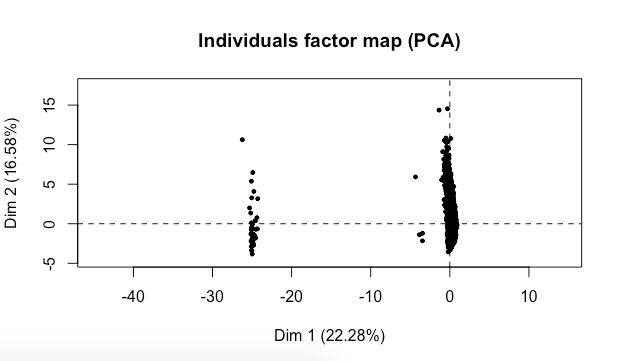
\includegraphics[width=\textwidth]{Seperate.png}

\section{Perform a PCA taking into account also supplementary variables}
Supplementary variables and individuals are not used for the determination of the principal components. Their coordinates are predicted using only the information provided by the performed principal component analysis on active variables/individuals.

The clustering looks pretty clear from this.

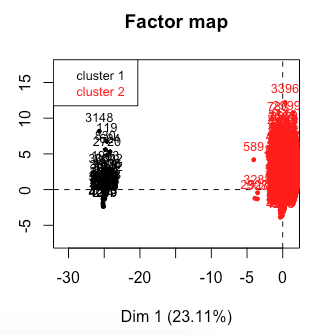
\includegraphics[width=\textwidth]{Cluster.png}
42 points belong to cluster 1, with 4391 in the 2nd cluster. This is forcing the clear two clusters. This 1st cluster is very small and could be considered unhelpful, unless these refer to outliers.

\label{my-label}
\begin{tabular}{lll}
       &       Eta2  &  P-value \\
Dim.1 & 0.9890591535 & 0.00000000 \\
Dim.2 & 0.0008660378 & 0.05008404
\end{tabular}

\section{More supplements}
The following variables correlate strongly with Fare\_Amount without being directly related to the fare amount.
\begin{itemize}
\item Fare\_Amount - 7
\item Trip\_time\_seconds - 17
\item RateCodeNF - 21
\item RateCodeStandard - 22
\item Trip\_type\_Dispatch - 26
\item Trip\_type\_street\_hail - 27
\end{itemize}

From my early investigation I only found two clusters, one cluster representing what I believe to be outliers, and the other normal data.

My mistake before was not involving other supplementaries in the clustering.

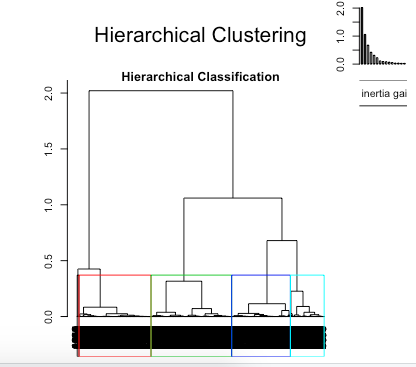
\includegraphics[width=\textwidth]{HierarchalClustering.png}
The colored boxes in the above graph represent the 5 different clusters, it is difficult to see the narrow black square on the far left, these are the outliers we clustered before. You can also see the clear different collections of data. And the graph below shows the new clusters.

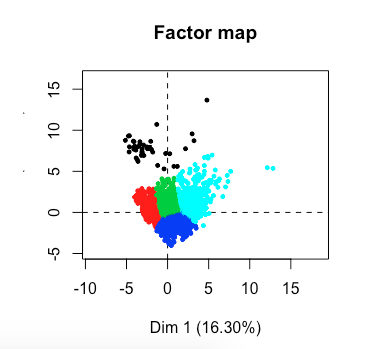
\includegraphics[width=\textwidth]{NewClusters.png}

The below table shows the split of clusters, with black, red, green, dark blue, light blue corresponding to 1,2,3,4,5. As you can see from our previous clustering we still have 42 outliers so the outliers class is still classified.

\begin{tabular}{lllll}
  1  &  2 &   3  &  4  &  5 \\
  42 & 1424 & 1069 & 1378 & 520
\end{tabular}

Next I have tried to come up with 5 plain English ways of describing these clusters. I have come up with the following.
\begin{itemize}
\item 1 - Outliers
\item 2 - Cheap Street hail, Negotiated Fares
\item 3 - Average trips
\item 4 - Expensive Street hail, Negotiated Fares
\item 5 - Expensive ,long, trips
\end{itemize}

\end{document}
